\subsection{Singleton}
\subsubsection{Định nghĩa}
Singleton là một Creational Pattern cho phép chúng ta chỉ có duy nhất một đối tượng được khởi tạo và sử dụng xuyên suốt chương trình của một class.
\subsubsection{Cách sử dụng}
Thông thường, các trường hợp có thể sử dụng Singleton như sau:
\begin{itemize}
    \item Khi bạn chỉ muốn có một đối tượng duy nhất của một lớp và muốn truy cập đến nó từ mọi nơi trong ứng dụng.
    \item Khi việc tạo lại đối tượng từ đầu mất thời gian và tài nguyên, và bạn muốn tái sử dụng đối tượng đã có.
\end{itemize}
\subsubsection{Cấu trúc}
Để có thể dễ dàng thực thi Singleton Pattern, ta thực hiện theo các bước sau:
\begin{itemize}
    \item 1. Để constructor private để ngăn các objects khác sử dụng từ khóa \textbf{new} với class Singleton.
    \item 2. Tạo một phương thức khởi tạo static mới để thay thế vai trò của constructor. Phương thức này gọi hàm constructor private để khởi tạo đối tượng và lưu đối tượng đó dưới dạng static. Tất cả các lần gọi tiếp theo đều trả về đối tượng đã được tạo static này.
\end{itemize}
\begin{center}
    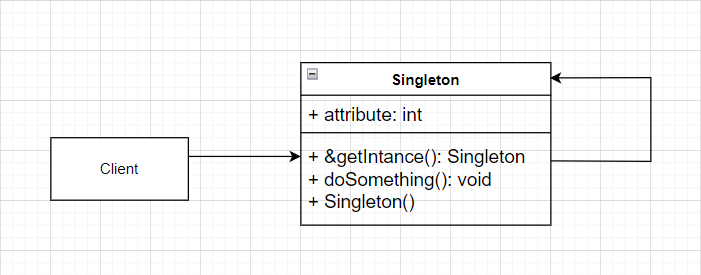
\includegraphics[]{image/creational/sso.png}
\end{center}
Các thành phần chính:
\begin{itemize}
    \item Các class khởi tạo đối tượng duy nhất chỉ định hàm constructor về private.
\end{itemize}
\subsubsection{Ưu điểm và Nhược điểmđiểm}
Ta thường thấy các ưu nhược điểm sau:\\\\
Ưu điểm:
\begin{itemize}
    \item Singleton đảm bảo rằng chỉ có một đối tượng duy nhất của lớp tồn tại trong suốt vòng đời của ứng dụng. Điều này đảm bảo rằng mọi truy cập đến đối tượng này đều nhận được cùng một thể hiện.
    \item Vì Singleton có phạm vi toàn cục trong ứng dụng, bạn có thể truy cập đến nó từ mọi nơi trong mã của bạn. Điều này giúp bạn dễ dàng chia sẻ thông tin và trạng thái giữa các phần khác nhau của ứng dụng.
    \item Singleton giúp bạn tiết kiệm tài nguyên bằng cách tái sử dụng một đối tượng đã có thay vì tạo ra một đối tượng mới mỗi khi cần sử dụng.
\end{itemize}
Nhược điểm:
\begin{itemize}
    \item Do Singleton tồn tại trong suốt vòng đời của ứng dụng, việc kiểm tra và kiểm soát đối tượng Singleton có thể trở nên khó khăn..
    \item Singleton có thể gây ra xung đột trong môi trường đa luồng hoặc trong trường hợp nhiều luồng cố gắng truy cập và sửa đổi đối tượng Singleton cùng một lúc. Cần phải chú ý đến việc đồng bộ hóa để tránh xung đột.
\end{itemize}
\subsubsection{Code}
\begin{itemize}
    \item Ta có một đối tượng duy nhất chỉ được khởi tạo một lần (class Singleton), lưu ý, ta để constructor ở trạng thái private.
    \item Ở class Singleton, ta có một phương thức static là getInstance() để kêu đối tượng được khởi tạo ban đầu ở mọi nơi trong code của chúng ta.
\end{itemize}
\begin{lstlisting}
#include <iostream>

using namespace std;

class Singleton
{
public:
    int attribute = 0;

public:
    static Singleton &getInstance()
    {

        static Singleton instance; // static local variable
        return instance;
    }

    void doSomething()
    {
        attribute++;
        cout << "attribute: " << attribute << endl;
    }

private:
    Singleton()
    {
        // private constructor to prevent direct instantiation
        cout << "Creating Singleton instance..." << endl;
    }

    ~Singleton()
    {
        // private destructor to prevent deletion of the instance
        cout << "Destroying Singleton instance..." << endl;
    }

    // private copy constructor and assignment operator to prevent cloning
    Singleton(const Singleton &) = delete;
    Singleton &operator=(const Singleton &) = delete;
};

int main()
{
    Singleton &singleton = Singleton::getInstance();
    singleton.doSomething();
    Singleton &singleton2 = Singleton::getInstance();
    singleton2.doSomething();

    return 0;
}

\end{lstlisting}
Ở hàm main, ta đầu tiên tạo ra đối tượng singleton, và thực hiện việc cộng biến lên 1 đơn vị. Sau đó, ta tiếp tục khởi tạo đối tượng mới tuy nhiên vẫn là gọi lại đối tượng cũ, và sau đó là thực hiện hành vi cộng biến lên 1 đơn vị và kết quả cho ra sẽ là 2.\\
\newline
\textbf{Kết quả:}
\begin{lstlisting}
Creating Singleton instance...
attribute: 1
attribute: 2
Destroying Singleton instance...
\end{lstlisting}